\documentclass[12pt]{article}
\usepackage[utf8]{inputenc}
\usepackage[spanish]{babel}
\decimalpoint
\usepackage{amsmath}
\usepackage{amsthm}
\usepackage{amssymb}
\usepackage{graphicx}
\usepackage[margin=0.9in]{geometry}
\usepackage{fancyhdr}
\usepackage[inline]{enumitem}
\usepackage{float}
\usepackage{cancel}
\usepackage{bigints}
\usepackage{color}
\usepackage{xcolor}
\usepackage{listings}
\usepackage{listingsutf8}
\usepackage{algorithm}
\usepackage{tocloft}
\usepackage[none]{hyphenat}
\usepackage{graphicx}
\usepackage{grffile}
\usepackage{tabularx}
\usepackage[nottoc,notlot,notlof]{tocbibind}
\renewcommand{\cftsecleader}{\cftdotfill{\cftdotsep}}
\pagestyle{fancy}
\setlength{\headheight}{15pt} 
\lhead {Mecanismos  de sincronización de procesos en Linux y Windows (semáforos)}
\rhead{\thepage}
\lfoot{Sistemas Operativos}
\renewcommand{\footrulewidth}{0.5pt}
\setlength{\parskip}{0.5em}
\newcommand{\ve}[1]{\overrightarrow{#1}}
\newcommand{\abs}[1]{\left\lvert #1 \right\lvert}
\definecolor{pblue}{rgb}{0.13,0.13,1}
\definecolor{pgreen}{rgb}{0,0.5,0}
\definecolor{pred}{rgb}{0.9,0,0}
\definecolor{pgrey}{rgb}{0.46,0.45,0.48}
\lstset{tabsize=1}
\bibliographystyle{IEEEtran}
\usepackage{listings}
\definecolor{dkgreen}{rgb}{0,0.6,0}
\definecolor{gray}{rgb}{0.5,0.5,0.5}
\definecolor{mauve}{rgb}{0.58,0,0.82}

\usepackage{hyperref}
\usepackage{listings}
\lstdefinestyle{customc}{
  belowcaptionskip=1\baselineskip,
  numbers=left,                   % where to put the line-numbers
  numberstyle=\tiny\color{gray},  % the style that is used for the line-numbers
  stepnumber=1,   
  breaklines=true,
  xleftmargin=\parindent,
  language=C,
  showstringspaces=false,
  basicstyle=\footnotesize,
  keywordstyle=\bfseries\color{green!40!black},
  commentstyle=\itshape\color{purple!40!black},
  identifierstyle=\color{blue},
  stringstyle=\color{orange},
}

\lstdefinestyle{customasm}{
  belowcaptionskip=1\baselineskip,
  frame=L,
  xleftmargin=\parindent,
  language=[x86masm]Assembler,
  basicstyle=\footnotesize\ttfamily,
  commentstyle=\itshape\color{purple!40!black},
}

\lstset{escapechar=@,style=customc}
\begin{document}
		\begin{titlepage}
			\begin{center}
				% Upper part of the page. The '~' is needed because \\
				% only works if a paragraph has started.
				\noindent
				\begin{minipage}{0.5\textwidth}
					\begin{flushleft} \large
					
\includegraphics[width=0.3\textwidth]{Imagenes/ipn.png}
					\end{flushleft}
				\end{minipage}%
				\begin{minipage}{0.55\textwidth}
					\begin{flushright} \large
			       	
\includegraphics[width=0.7\textwidth]{Imagenes/escom.png}
					\end{flushright}
				\end{minipage}
				\textsc{\LARGE Instituto Politécnico Nacional}\\[0.5cm]
				\textsc{\Large Escuela Superior de Cómputo}\\[1cm]
				% Title
				{ \huge Práctica No.7 \\[1cm] }
				{\huge Mecanismos  de sincronización de procesos en Linux y Windows (semáforos)\\[1cm]}
				{ \Large Unidad de aprendizaje: Sistemas Operativos} \\[1cm]
				{ \Large Grupo: 2CM8 } \\[1cm]
				\noindent
				\begin{minipage}{0.5\textwidth}
					\begin{flushleft} \large
						\emph{Integrantes del equipo:}\\
						\begin{tabular}{ll}
					     Domínguez Morán Joaquín\\
					     Carrillo Balcazar Eduardo Yair\\
					     Ruiz López Luis Carlos\\
					\end{tabular}
					\end{flushleft}
				\end{minipage}%
				\begin{minipage}{0.5\textwidth}
					\begin{flushright} \large
						\emph{Profesor:} \\
						Jorge Cortes Galicia 
					\end{flushright}
				\end{minipage}
				
				\vfill
				% Bottom of the page
				{\large 02 de diciembre de 2018}
			\end{center}
		\end{titlepage}
		
\section{Competencias.}
El alumno comprende el funcionamiento de los mecanismos de sincronización entre procesos cooperativos utilizando los semáforos como árbitros de acceso para el desarrollo de aplicaciones cooperativas tanto en el sistema operativo Linux como Windows.
\section{Desarrollo.}
    \subsection{Linux}
    \begin{enumerate}
        \item Acontinuación se explica el funcionamiento de las siguientes funciones: 
        \begin{itemize}
            \item \textbf{semget():Obtiene un identificador del conjunto de semáforos de System V}\\
            \begin{itemize}
                 \item \textbf{Argumentos}\\
                    #include$<$sys/types.h$>$ \\
                    #include$<$sys/ipc.h$>$ \\
                    #include$<$sys/sem.h$>$ \\
                    int semget ( clave key\_t , int nsems , int semflg );\\
                    \begin{itemize}
                         Identificador asociado a la \textbf{key} de argumento .Se puede usar para obtener el identificador de un conjunto de semáforos creado anteriormente (cuando \textbf{semflg} es cero y la clave no tiene el valor IP\_PRIVATE ) o para crear un nuevo conjunto. \\
                         Se crea un nuevo conjunto de semáforos nsems si la clave tiene el valor IPC\_PRIVATE o si ningún conjunto de semáforos existente está asociado con la clave y IPC\_CREAT está especificado en \textbf{semflg}.
                        Al crear un nuevo conjunto de semáforos, semget () inicializa la estructura de datos asociada al conjunto , semid\_ds de la siguiente manera: sem\_perm.cuid y sem\_perm.uid se establecen en la identificación de usuario efectiva del proceso de llamada. sem\_perm.cgid y sem\_perm.gid se establecen en la identificación de grupo efectiva del proceso de llamada.

                        Los 9 bits menos significativos de sem\_perm.mode se establecen en los 9 bits menos significativos de semflg . sem\_nsems se establece en el valor de nsems . sem\_otime se establece en 0. sem\_ctime se establece en la hora actual. 
                        El argumento nsems puede ser 0 (no me importa) cuando no se está creando un conjunto de semáforos . De lo contrario, nsems debe ser mayor que 0 y menor o igual que la cantidad máxima de semáforos por conjunto de semáforos.

                    \end{itemize}
                    \item \textbf{Retorno:}\\
                    Si tiene éxito, el valor de retorno será el identificador del conjunto de semáforos (un entero no negativo), de lo contrario, se devuelve -1, con errno indicando el error.
            \end{itemize}
            \item \textbf{semop(): Realiza operaciones del semáforo del Sistema V}
                \begin{itemize}
                    \item \txtbf{Argumentos:}\\
                    #include$<$sys/types.h$>$\\ 
                    #include$<$sys/ipc.h$>$ \\
                    #include$<$sys/sem.h$>$ \\
                    int semop (int semid , struct sembuf * SOPs , size\_t nsops ); 
                int semtimedop (int semid , struct sembuf * sops , size\_t nsops ,const struct timespec * tiempo de espera );\\
                    \begin{itemize}
                        Cada semáforo en un conjunto de semáforos del Sistema V tiene lo siguientes valores asociados:\\
                        \\
                            unsigned short  semval;   /* valor de semáforo  */\\
                            unsigned short  semzcnt;  /* # esperando cero  */\\
                            unsigned short  semncnt;  /* # espera por incremento */\\
                            pid\_t           sempid;\\
                            El PID del proceso que finaliza el semop () realiza operaciones en semáforos seleccionados en el conjunto indicado  por semid . Cada uno de los nsops elementos en el array apuntado por sops es una estructura que especifica una operación a ser realizada en un solo semáforo. \\. Los elementos de esta estructura son de tipo struct sembuf, que contiene los siguientes miembros: \\

                               unsigned short sem\_num;    /*número de semáforo*/ \\
                               short sem\_op;                    /*    operación de semáforo */ \\
                               short sem\_flg;                     /*   indicadores de operación*/ \\

                Los indicadores reconocidos en sem\_flg son IPC\_NOWAIT y SEM\_UNDO . Si una operación específica SEM\_UNDO , se deshará automáticamente cuando finalice el proceso.
                
                El conjunto de operaciones contenidas en sops se realiza en orden de ordenadas, y atómicamente, es decir, las operaciones se realizan como una unidad completa, o no se realizan en absoluto. El comportamiento de la llamada al sistema si no todas las operaciones se pueden realizar inmediatamente depende de la presencia del indicador IPC\_NOWAIT en los campos sem\_flg individuales , como se indica a continuación. 
                 
                Cada operación se realiza en el sem\_num semáforo -ésima del semáforo conjunto, donde el primer semáforo del conjunto está numerado 0.

                    \end{itemize}
                    \item \textbf{Retorno:}\\
                    Si tiene éxito, semop () y semtimedop () devuelven 0; de lo contrario, devuelven -1 con errno que indica el error.
                \end{itemize}
        \newpage
        \end{itemize}
        \item Capture, compile y ejecute el siguiente código:
        \lstinputlisting{Codigos/Linux/1.c}
        \begin{center}
            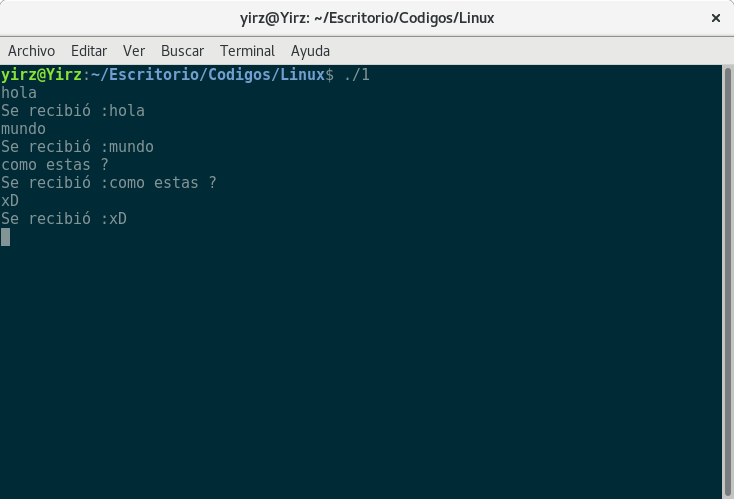
\includegraphics[scale=0.55]{Imagenes/Linux/1.png}
        \end{center}
    \end{enumerate}
    \newpage
\subsection{Windows}
    \begin{enumerate}
        \item Capture,compile y ejecute los siguientes códigos:
        
        \textbf{Padre:}
        \lstinputlisting{Codigos/Windows/Ejemplo/padre.c}
        
        \textbf{Hijo:}
        \lstinputlisting{Codigos/Windows/Ejemplo/hijo.c}
        \begin{center}
            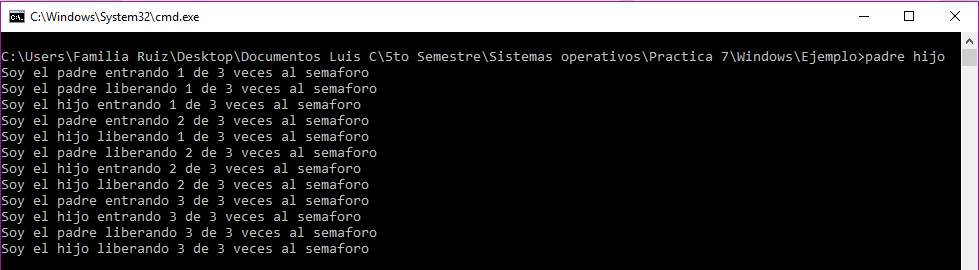
\includegraphics[scale=0.55]{Imagenes/Windows/ejemplo.PNG}
        \end{center}
        
    \end{enumerate}

\subsection{Programas Desarrollados}
    Programe la misma aplicación de la práctica 6 del punto 7  utilizando como máximo 3 renglones de memoria compartida de 400 bytes cada una para almacenar todas las matrices requeridas por la aplicación.
    \subsubsection{Linux}
    \begin{center}
        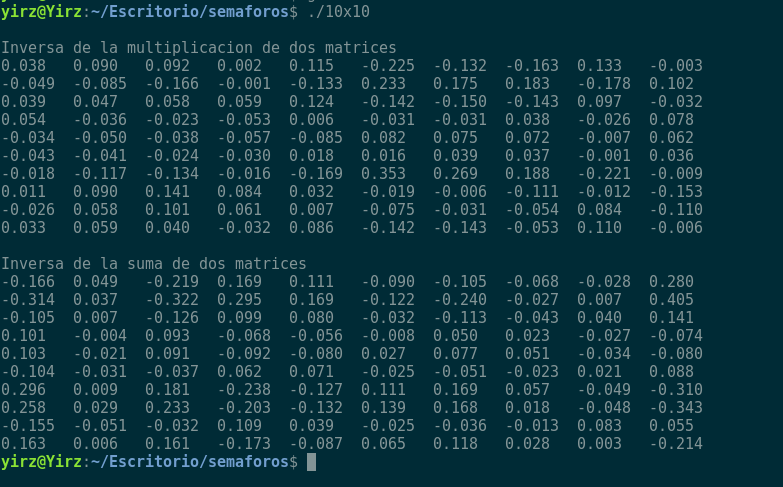
\includegraphics[scale=0.5]{Imagenes/Linux/semaforos.png}
    \end{center}
    \begin{center}
        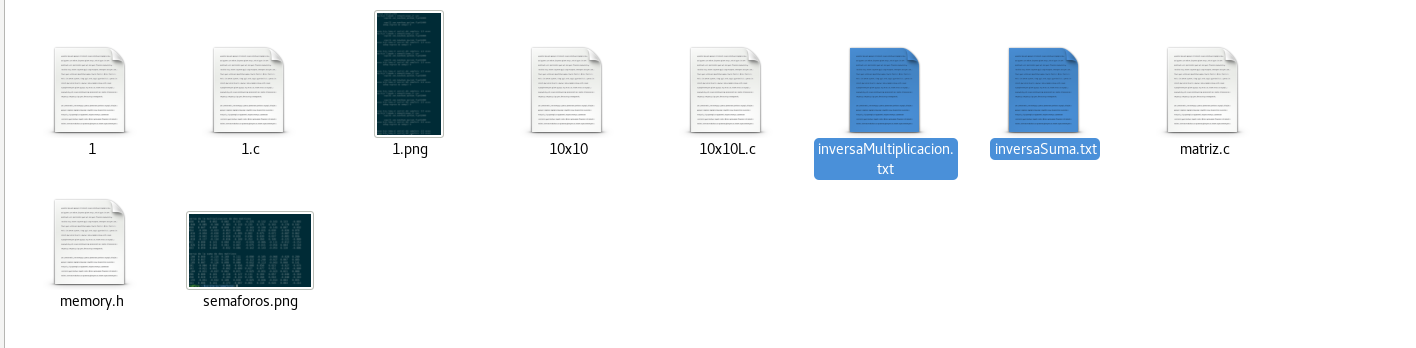
\includegraphics[scale=0.40]{Imagenes/Linux/semaforos2.png}
    \end{center}
    \subsubsection{Windows}
       \begin{center}
        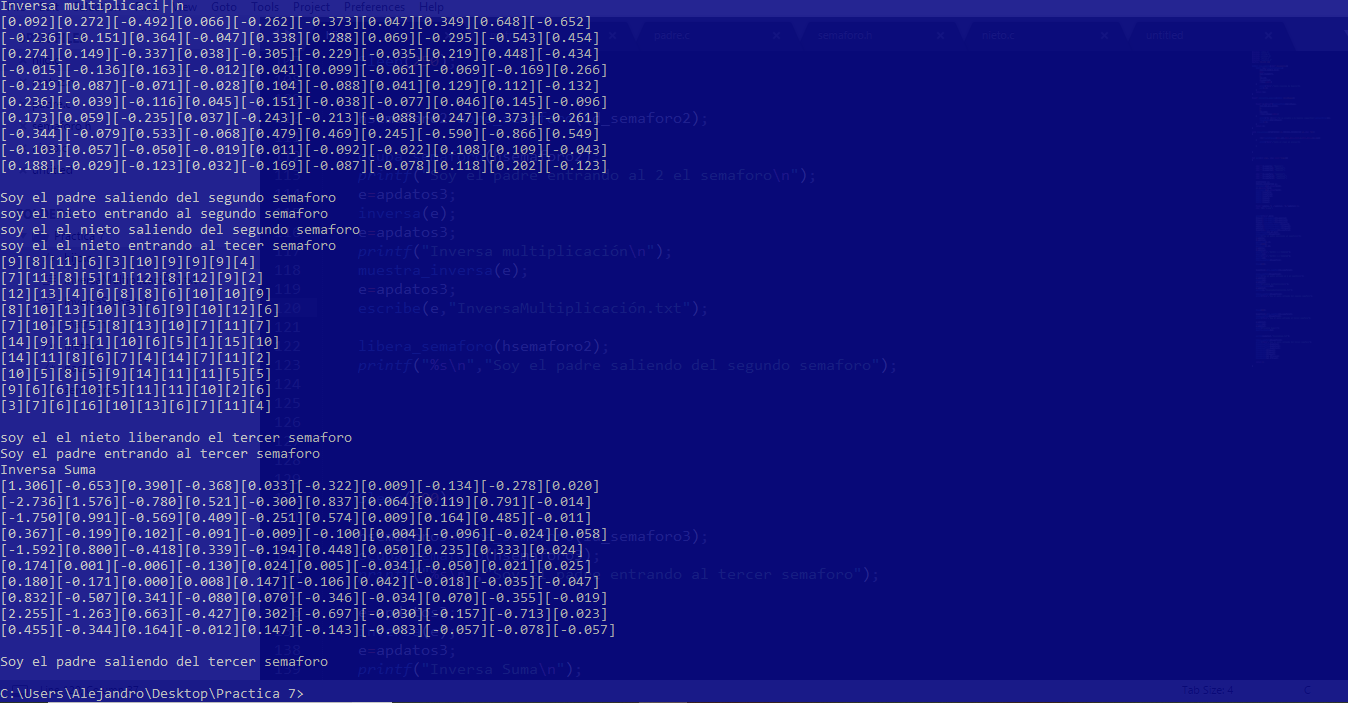
\includegraphics[scale=0.5]{Imagenes/Windows/semaforosW.png}
    \end{center}
    \begin{center}
        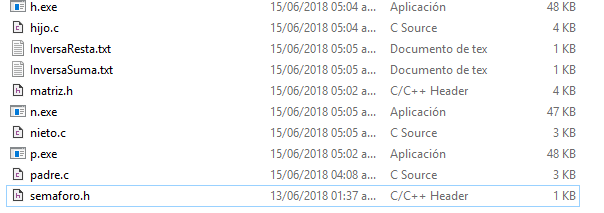
\includegraphics[scale=0.60]{Imagenes/Windows/semaforosW(1).png}
    \end{center}
    \begin{center}
        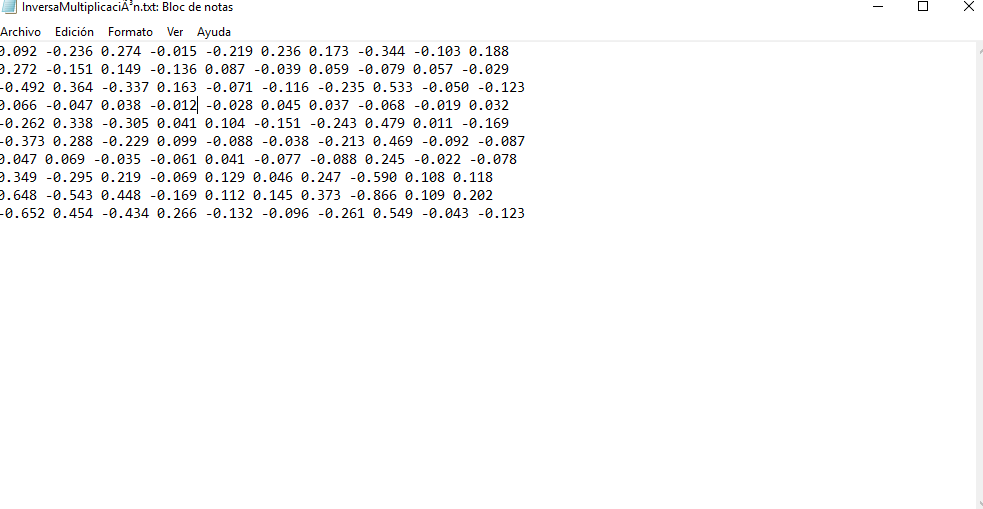
\includegraphics[scale=0.5]{Imagenes/Windows/semaforosW(2).png}
    \end{center}
    \begin{center}
        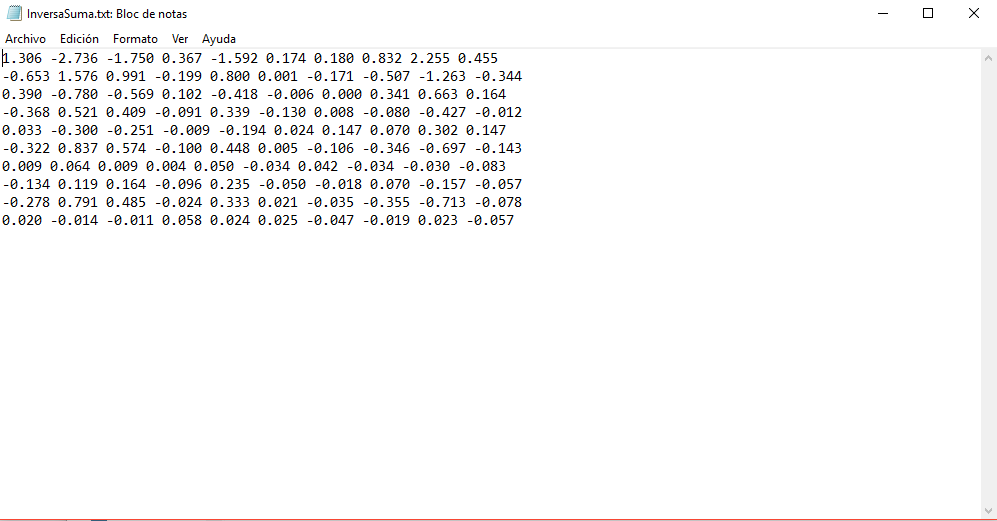
\includegraphics[scale=0.50]{Imagenes/Windows/semaforosW(3).png}
    \end{center}
\subsection{Código Fuente.}
   \subsubsection{Linux}
   \begin{itemize}
       \item Código matriz
       \lstinputlisting{Codigos/Linux/matriz.c}
       \item Código donde se crea la memoria compartida
       \lstinputlisting{Codigos/Linux/memory.h}
       \item Código del programa principal
       \lstinputlisting{Codigos/Linux/10x10L.c}
   \end{itemize}
   
   \subsection{Windows}
    \begin{itemize}
       \item Código matriz
       \lstinputlisting{Codigos/Windows/P4/matriz.h}
       \item Código del semaforo
       \lstinputlisting{Codigos/Windows/P4/semaforo.h}
       \item Código del padre
       \lstinputlisting{Codigos/Windows/P4/padre.c}
       \item Código del hijo
       \lstinputlisting{Codigos/Windows/P4/hijo.c}
       \item Código del nieto
       \lstinputlisting{Codigos/Windows/P4/nieto.c}
   \end{itemize}
   
  
   


\section{Observaciones.}

Primeramente podemos observar que la primera vez que un proceso usa el semáforo, este tiene valor 1, por lo que pasa a cero y el proceso puede acceder al recurso. Si durante ese tiempo otro proceso quiere acceder también, al usar el semáforo, este tiene valor cero, por lo que el sistema operativo deja de darle ciclos de CPU. Cuando el primer proceso ha terminado, libera el recurso, con lo que el sistema operativo puede comprobar que el segundo proceso está esperando, por lo que le vuelve a dar ciclos. En este punto, el proceso sigue como si nunca hubiese sido detenido. 

Otra utilización de los semáforos  que pdemos observar, es cuando uno o más procesos tienen que esperar a que otro halla terminado una tarea. Para ello, el primer proceso borra el semáforo y con una primitiva adecuada se pone a esperar a que el semáforo se active . Mientras, el segundo proceso va trabajando, y cuando termina lo que tiene que hacer, activa el semáforo, con lo que el primer proceso vuelve a ponerse en marcha, sin haber desperdiciado ciclos de CPU. 

\section{Análisis Crítico.}

La sincronizacion entre procesos es necesaria para prevenir y/o corregir errores de sincronizacion debidos al acceso concurrente a recursos compartidos, tales como estructuras de datos o dispositivos de E/S, de procesos contendientes. La sincronizacion entre procesos tambien permite intercambiar senales de tiempo (ARRANQUE/PARADA) entre procesos cooperantes para garantizar las relaciones especificas de precedencia impuestas por el problema que se resuelve.
Sin una sincronizacion adecuada entre procesos, la actualizacion de variables compartidas puede inducir a errores de tiempo relacionados con la concurrencia que son con frecuencia dificiles de depurar. Una de las causas principales de este problema es que procesos concurrentes puedan observar valores temporalmente inconsistentes de una variable compartida mientras se actualizan. una aproximacion para resolver este problema es realizar actualizaciones de variables compartidas de manera mutuamente exclusiva. Se pueden mejorar permitiendo que a lo mas un proceso entre a la vez en la seccion critica de codigo en la que se actualiza una variable compartida o estructura de datos en particular.

\section{Conclusiones.}

El uso de semáforos es de trasendencia en los sistemas operativos, sabiendo que es un método para restringir o permitir el acceso a recursos compartidos por lo cual nos permite un mayor control sobre lo que puede o no hacer nuestro programa en un entorno en el que se ejecutarán varios procesos concurrentemente. Tomando en cuenta que un tipo simple de semáforo es el binario, que puede tomar solamente los valores 0 y 1. Se inicializan en 1 y son usados cuando sólo un proceso puede acceder a un recurso a la vez. Aprovechando que se pueden sincronizar dos o más hilos o procesos, de modo que su ejecución se realice de forma ordenada y sin conflictos entre ellos.


\end{document}